\chapter{Discussion} \label{ch:discussion}

\section{Trends in experiments}
In general we found that for the synthetic datasets with multiple object instances, the best localization results are obtained by the Score-CAM for VGG16-GAP and VGG16 and by Grad-CAM++ for ResNet-50. Grad-CAM++ also performs best for the ImageNet dataset, both on VGG16-GAP and on ResNet-50. These quantitative evaluations confirm the promising results for multi-instance visualization observed by Wang \textit{et al.} \cite{wang2020score} and Chattopadhay \textit{et al.} \cite{chattopadhay2018grad}.

Score-CAM is not performing as good as the other localization methods for the ImageNet datasets, both on VGG16-GAP and on ResNet-50. As the majority of images in the ImageNet dataset has only one object instance of the target class, the promising results for multi-instance detection by Score-CAM do not weigh in the localization results for ImageNet. The fact that Score-CAM computes its score maps based on the score of the target class (Wang \textit{et al. \cite{wang2020score}} and because the classification accuracy for the ImageNet dataset is much lower than for the synthetic datasets, may further explain why Score-CAM is not performing as well for ImageNet as for the synthetic datasets.


In the iterative localization experiments, we found that the Grad-CAM++ and Score-CAM localization methods are best in improving the localization recall when compared to the non-iterative baseline results. When comparing all localization methods, we observed that the lower the baseline results are, the more can be gained in recall improvement by applying the iterative approach. However, the larger the improvement in recall, the larger the precision drop for these methods. This can be explained by looking at the iterative strategies that give the best recall improvements. They tend to generate more predictions, both true and false positives. A more detailed discussion on which iterative methods provide the best results is provided in section \ref{dis:iterative_localizaiton}.

\section{Precision and recall correlation with object instances}
When observing the multi-instance localization precision and recall values in our experiments, we found that both metrics decrease as the number of object instances in images increases. This was observed for all networks (VGG16-GAP, VGG16, ResNet-50), non-regularized and MinMaxCAM regularized models and datasets (synthetic, ImageNet datasets partitioned by number of object instances).

For the ImageNet dataset, we don't see the mentioned correlation between precision and number of object instances in images, for those datasets that have more than four object instances per image. As there are more object instances in an image, the more areas are expected to be activated areas in the score maps. When the distance between these areas becomes smaller for more instances, the localization methods may localize groups of instances as a single instance, which will impact recall but not not precision.

For the synthetic datasets, we observed that pixel average precision (PxAP) doesn’t drop as significantly as the MaxBoxAccV3 metrics for images with increasing number of object instances. As the PxAP measures localization at pixel level and MaxBoxAccV3 metrics at bounding box level, it's reasonable to assume that a mismatch between predicted and ground truth object localization, results in a less severe penalty for a pixel level metric.

\section{Non-regularized versus regularized models}
We observed for non-regularized VGG16-GAP and ResNet-50 models evaluated on synthetic datasets and ImageNet, that localization performance of the CAM method could be improved by Grad-CAM++ or Score-CAM.

Networks trained with MinMaxCAM-regularization that give an improvement for CAM-based localization, give an even better result for Grad-CAM++ or Score-CAM. This means that the localization trends from the non-regularized model thus transfer to the MinMaxCAM-regularized model.

\section{Threshold calibration}
Different localization methods exhibit different localization performance distributions, as illustrated in Fig. \ref{fig:boxacc_resnet50_imagenet}. Here we show the box accuracy (BoxAccV2 as defined in equation \ref{eq:boxaccv2}) using different localization methods for the ResNet-50 network on the ImageNet validation dataset. We use a BoxAcc plot to illustrate box accuracy in function of the score map threshold. Fig. \ref{fig:boxacc_resnet50_imagenet} clearly shows that each localization method has a different BoxAcc distribution. Fixing the score map threshold at a single pre-defined value, could lead to increased performance of some methods and to decreased performance for others. 

The threshold-independent localization metric MaxBoxAccV3 recall (MaxBoxAccV3 in short) is then the maximum value of the BoxAcc metric in the plot. The optimal score map threshold is the score map threshold for the maximum box accuracy. We observe that the localization methods have different optimal score map thresholds, but the MaxBoxAccV3 values are not significantly different. This provides an explanation of the limited differences between localization methods for MaxBoxAccV3 recall as observed in Table \ref{tab:metrics_resnet50_imagenet}.

\begin{figure}[ht]
    \begin{center}       
    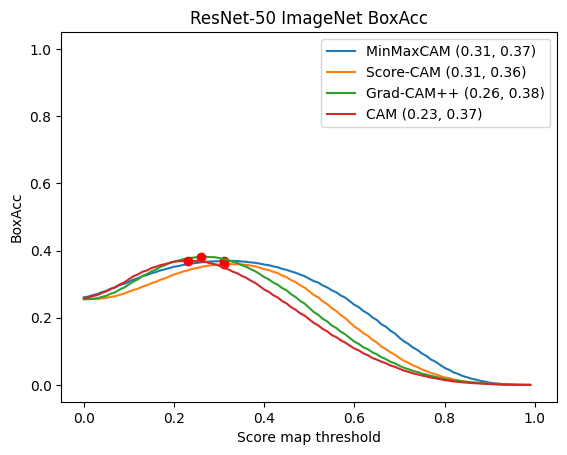
\includegraphics[width=0.7\textwidth]{fig_boxacc_resnet50_imagenet.png}
    \caption[BoxAcc (IoU 50)for ResNet-50 on ImageNet]{Performance at varying operating thresholds. BoxAcc($\tau$) versus score map threshold $\tau$ at IoU threshold 50 for ResNet-50 on ImageNet.}
    \caption*{Source: Author}
    \label{fig:boxacc_resnet50_imagenet}
    \end{center}
\end{figure}

\section{Classification versus localization accuracy}
When comparing classification accuracy with localization accuracy (MaxBoxAccV3 recall) during training, we observed that there is a correlation between both metrics. Fig. \ref{fig:loc_vs_acc_vgg16_gap_cam_synthetic} illustrates that classification accuracy and CAM localization accuracy (MaxBoxAccV3 recall) for VGG16-GAP on each of the validation synthetic datasets, improve during the early epochs of training, until both metrics start converging.

A question is then which checkpoint during training is suitable for localization evaluation? Choe \textit{et al.} \cite{choe2020evaluating} argue that in many cases, the best localization performances are achieved before convergence, that at early epochs, the localization can fluctuate a lot and thus, peak performance is noise rather than real performance. Fig. \ref{fig:loc_vs_acc_resnet50_cam_d1b} illustrates such case for the CAM localization method on ResNet-50 for the d1b synthetic dataset. We clearly see that the maximum value for MaxBoxAccV3 is reached during the early training epochs, and drops around epoch 10 before converging.

To avoid measuring noise, we use an early stop criterion that ends model training when classification accuracy has not improved the best accuracy for five consecutive training epochs. We then take as localization accuracy the value computed at the last epoch on the validation dataset.

\begin{figure}[ht]
\begin{center}
    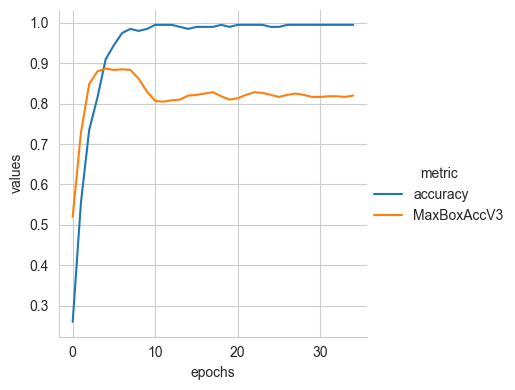
\includegraphics[width=0.6\textwidth]{images/fig_loc_vs_acc_resnet50_cam_d1b.png}
    \caption[Classification versus CAM localization accuracy on ResNet-50 for d1b dataset]{Classification versus CAM localization accuracy on ResNet-50 for d1b dataset.}
    \caption*{Source: Author}
    \label{fig:loc_vs_acc_resnet50_cam_d1b}
\end{center}
\end{figure}

\section{Iterative localization} \label{dis:iterative_localizaiton}
The results of the iterative localization experiments in section \ref{sec:exp_loc_improvements} show that localization recall can be improved using the iterative approach on all localization metrics. Depending on the mask strategy, merge strategy and chosen stop criterion, recall can be improved substantially. In most cases, recall improvement comes at the cost of precision loss when compared with the baseline.

The two parameters that are most important for improving recall, are the merge strategy and the iteration stop criterion. This is understandable as these two parameters directly determine whether predicted bounding boxes will be added to the list of bounding boxes predicted during previous iterations. 

For the synthetic datasets with multiple object instances and in the ImageNet dataset, the experiments using the 'add' merge strategy and iteration stop threshold 1.0 show the most substantial gain in recall but at a large impact on precision. It is easy to see that in this scenario, each iteration can add more bounding boxes, potentially increases matches or mismatches between predicted and ground truth bounding boxes, hence increasing recall in the former and decreasing precision in the latter case.

The experiments with the large and diverse ImageNet dataset shows that there is quite some room for improving localization recall. However, the current iterative approach stills suffers from substantial loss in precision. Precision for the iterative approach is bad because of the bias in ImageNet to images with single object instance. We expect the results to be more in line with other experiments for synthetic dataset if the iterative localization would be done on the ImageNet dataset split by object instance count. We see this as future work.

In our current iterative localization approach, we use bounding boxes predicted in previous iterations as image masks to predict new boxes. As future work it would be interesting to evaluate using the more fine-grained score map as an image mask for improving precision.